%**************************************************************%
%                     File Name: main.tex                      %
%                                                              %
%    37th International Ocean and Polar Engineering Conference %
%                        (ISOPE-2027)                          %
%  Adapted from Official ISOPE LaTeX Template (M. Kashiwagi)   %
%**************************************************************%
\documentclass[11pt,fleqn,letterpaper]{article}
\usepackage[T1]{fontenc}
\usepackage{graphicx}
\usepackage{amsmath,amssymb}
\usepackage{txfonts}
\usepackage{bm}
\usepackage{booktabs}
\usepackage{array}
\usepackage{multirow}
\usepackage[hidelinks]{hyperref}

%**************************************************************%
%                   File Name: deffile.tex                     %
%                                                              %
%  ISOPE Conference Paper LaTeX Style Definitions              %
%  Adapted from the Official ISOPE Template by M. Kashiwagi    %
%  Updated for standard pdfLaTeX / XeLaTeX / Tectonic &        %
%  US Letter (8.5in x 11in) ISOPE Proceedings Camera-Ready     %
%**************************************************************%
\makeatletter
%%%%%%%%%%%%%%%%%%%%%%% Style of Footer %%%%%%%%%%%%%%%%%%%%%%%%%%%%%%
\def\ps@isopefoot{\let\@mkboth=\@gobbletwo
 \def\@oddhead{}
 \def\@evenhead{}
 \def\@oddfoot{\hbox to \textwidth
   {\footnotesize {Paper No.\,2027-\papernumber} \hfil
   {\firstauthorname} \hfil {Page number:\ \thepage\ of\ \totalpage}}}
 \def\@evenfoot{\hbox to \textwidth
   {\footnotesize {Paper No.\,2027-\papernumber} \hfil
   {\firstauthorname} \hfil {Page number:\ \thepage\ of\ \totalpage}}}
}%
%---------------------------------------------------------------
\setcounter{topnumber}{4}
\def\topfraction{0.95}
\setcounter{bottomnumber}{3}
\def\bottomfraction{0.90}
\setcounter{totalnumber}{6}
\def\textfraction{0.05}
\def\floatpagefraction{0.85}
%
\setcounter{dbltopnumber}{4}
\def\dbltopfraction{0.95}
\def\dblfloatpagefraction{0.85}
%---------------------------------------------------------------
% Clean ISOPE caption formatting (flush baseline, zero overfull hbox)
\long\def\@makecaption#1#2{%
  \vskip 4\p@
  \footnotesize\baselineskip=9.8pt
  \sbox\@tempboxa{#1 #2}%
  \ifdim \wd\@tempboxa >\hsize
    \noindent #1 #2\par
  \else
    \global \@minipagefalse
    \hb@xt@\hsize{\hfil\box\@tempboxa\hfil}%
  \fi
  \vskip 2\p@
}
%--------------------------------------------------------
\def\fnum@figure{{\footnotesize\bf Fig.\,\thefigure.}}
\def\fnum@table{{\footnotesize\bf Table\,\thetable.}}
%
%%%%%%%%%%%%%%%%%%%%%%%%%%%%%%%%%%%%%%%%%%%%%%%%%%%%%%%%%%%%%%%%%%%%%%
\def\thesection{}
\def\thesubsection{}
\def\thesubsubsection{}
%
\def\section{\@startsection{section}{1}{\z@}
{1.4ex plus .2ex minus .15ex}{0.65ex plus .1ex}{\small\bf}}
\def\subsection{\@startsection{subsection}{2}{\z@}
{1.0ex plus .15ex minus .15ex}{0.45ex plus .1ex}{\footnotesize\bf}}
\def\subsubsection{\@startsection{subsubsection}{3}{\z@}
{0.8ex plus .15ex minus .1ex}{0.35ex plus .1ex}{\footnotesize\it}}
%
\def\paragraph{\@startsection{paragraph}{4}{\z@}
{0.8ex plus .2ex minus .1ex}{-1em}{\footnotesize\bf}}
\def\subparagraph{\@startsection{subparagraph}{4}
{\parindent}{0.8ex plus .2ex minus .1ex}{-1em}{\footnotesize\it}}
%---------------------------------------------------------------------
\def\@cite#1#2{\,[{\hbox{#1\if@tempswa , #2\fi}}]}
%
\makeatother
%---------------------------------------------------------------
% Flush-left ISOPE unnumbered section commands
\def\jsection#1{\section*{\uppercase{#1}}}
\def\jsubsection#1{\subsection*{#1}}
\def\jsubsubsection#1{\subsubsection*{#1}}
%---------------------------------------------------------------
% Guard Japanese pLaTeX macro for full compatibility with pdfLaTeX / XeLaTeX / Tectonic
\providecommand{\autospacing}{}
\autospacing
%
\newcommand{\bdm}{\begin{displaymath}}
\newcommand{\edm}{\end{displaymath}}
\newcommand{\be}{\begin{equation}}
\newcommand{\ee}{\end{equation}}
\newcommand{\bea}{\begin{eqnarray}}
\newcommand{\eea}{\end{eqnarray}}
%
\newcommand{\bc}{\begin{center}}
\newcommand{\ec}{\end{center}}
\newcommand{\bfl}{\begin{flushleft}}
\newcommand{\efl}{\end{flushleft}}
\newcommand{\bfr}{\begin{flushright}}
\newcommand{\efr}{\end{flushright}}
\newcommand{\ds}{\displaystyle}
%---------------------------------------------------------------
\newcommand{\mbf}[1]{\mbox{\boldmath$#1$}}
\newcommand{\ubar}[1]{\overline{#1}}
\newcommand{\hs}{\hspace*{0.2mm}}
\newcommand{\npar}{\par\vspace*{4pt}}
%
% Hanging-indent ISOPE reference entry (author-year style, unnumbered)
\newcommand{\isoperef}[1]{%
  \par\noindent\hangindent=4.2mm\hangafter=1{\fontsize{7.4}{8.5}\selectfont #1}\par\vspace*{0.45mm}%
}
%
%%%%%%%%%%%%%%%%%%%%%%%%%%%%%%%%%%%%%%%%%%%%%%%%%%%%%%%%%%%%%%%
% Official ISOPE Letter-size (215.9mm x 279.4mm) layout geometry
\setlength{\textheight}  {243.0mm}
\setlength{\textwidth}   {191.9mm}
\setlength{\columnsep}   {8.9mm}
\setlength{\parindent}   {0.0mm}
\setlength{\parskip}     {2.6pt plus 0.6pt minus 0.3pt}
\setlength{\mathindent}  {0.0mm}
% Tight, balanced float spacing
\setlength{\floatsep}        {5pt plus 2pt minus 2pt}
\setlength{\textfloatsep}    {7pt plus 2pt minus 2pt}
\setlength{\intextsep}       {6pt plus 2pt minus 2pt}
\setlength{\dblfloatsep}     {5pt plus 2pt minus 2pt}
\setlength{\dbltextfloatsep} {7pt plus 2pt minus 2pt}
\setlength{\abovedisplayskip}{3.5pt plus 1pt minus 1pt}
\setlength{\belowdisplayskip}{3.5pt plus 1pt minus 1pt}
%
\newlength{\mybaselineskip}
\setlength{\mybaselineskip}{9.85pt}
\newlength{\myleftmargin}
\newlength{\mytopmargin}
%%%%%% For the US Letter size (ISOPE Format: 8.5in x 11in) %%%%
\setlength{\myleftmargin}  {12.0mm}
\setlength{\mytopmargin}   {10.5mm}
%%%%%%%%%%%%%%%%%%%%%%%%%%%%%%%%%%%%%%%%%%%%%%%%%%%%%%%%%%%%%%%
\setlength{\oddsidemargin} {-1in}
\setlength{\topmargin}     {-1in}
\addtolength{\oddsidemargin}{\myleftmargin}
\addtolength{\topmargin}    {\mytopmargin}
\setlength{\headheight}  { 0.0mm}
\setlength{\headsep}     { 8.0mm}
\setlength{\footskip}    {13.0mm}
%
\sloppy

\pagestyle{empty}

% Paper metadata (for optional review footer if \pagestyle{isopefoot} is enabled)
\newcommand{\papernumber}{TPC-XXX}
\newcommand{\firstauthorname}{Huang Ximing}
\newcommand{\totalpage}{8}

% Compact table column helper
\newcolumntype{C}[1]{>{\centering\arraybackslash}p{#1}}
\newcolumntype{L}[1]{>{\raggedright\arraybackslash}p{#1}}

%+-+-+-+-+-+-+-+-+-+-+-+-+-+-+-+-+-+-+-+-+-+-+-+-+-+-+-+-+-+-+-+-+
\begin{document}
\baselineskip \mybaselineskip
\twocolumn[{%
\par\vspace*{40.0mm}
\large\bc{\bf
Enhancing Aerodynamic Shape Optimization via Reinforcement Meta-Learning,\\
Large Language Models, and Likelihood-Free Bayesian Meta-Learning
}\ec
\par\vspace{1.5mm}\footnotesize\bc{\small\it
Huang Ximing\,$^{a}$, Xing Xiuqing\,$^{b}$, Zhang Xiaoqin\,$^{b}$, Kang Chang Wei\,$^{b}$
}\\[1.5mm]
$^{a}$\,College of Computing and Data Science, Nanyang Technological University, 50 Nanyang Ave, Singapore 639798\\
$^{b}$\,A*STAR Institute of Advanced Intelligence and Computing, 1 Fusionopolis Way, \#16-16, Connexis North Tower, Singapore 138632
\ec\par\vspace*{12.0mm}
}]

\footnotesize\par\noindent{\small\bf ABSTRACT}\par\vspace*{1.2mm}
\baselineskip \mybaselineskip
Aerodynamic shape optimization (ASO) of lifting sections and wind turbine blades is a high-dimensional, non-convex, strictly constrained black-box problem under severe evaluation budgets. While classical derivative-free optimizers use fixed hyperparameter schedules, emerging meta-optimization paradigms---reinforcement meta-learning (RL-Meta), large language model (LLM)-guided meta-control, and likelihood-free Bayesian meta-learning (MALIBO)---exploit prior optimization experience or physical reasoning differently. We conduct a rigorous, zero-leakage empirical audit of all three paradigms across a unified multi-fidelity benchmark bridging 2D airfoil design ($D=18$, NACA 0012 at held-out $Re=3.5\times 10^{6}, \alpha=3.5^\circ$, ten industrial geometric/moment constraints) and 3D NREL Phase VI wind turbine blade design ($D=63$, $V_\infty=7.0\,\text{m/s}, 72\,\text{rpm}$, 31 full-cosine blade element momentum sections, $C^1$ PCHIP/B-spline lofting, thrust cap $T \le 1.15\,T_0$) over 300 evaluations and 10 independent seeds.

In 2D, pure paired control-variate PPO RL-Meta (satisfying exact zero-action identity with untouched textbook defaults) improves all six derivative-free solvers (grand mean $L/D$: $180.87 \to 201.85$, $+11.6\%$), revealing a clear hyperparameter-sensitivity stratification: Py-BOBYQA ($+47.1\%$, $p<10^{-4}$) and SPSA ($+15.8\%$, $p=0.0154$) gain dramatically, CMA-ES ($+8.9\%$, $p=0.0047$) and DE ($+5.1\%$) gain steadily, while TuRBO ($+2.9\%$) and PSO ($+0.2\%$) remain strictly non-harmful. Comparing four paradigms on TuRBO, zero-leakage stagnation-adaptive LLM-Meta-TuRBO (\texttt{Qwen3.8-27B-FP8}) achieves top accuracy and efficiency in both 2D ($L/D = 227.40 \pm 13.41$, $+16.2\%$ vs.\ TuRBO, $p=0.0018$) and 3D ($P = 6.6664 \pm 0.0196\,\text{kW}$, $+9.49\%$ vs.\ baseline, $p=0.0014$ vs.\ TuRBO-1, $>3\times$ speedup, peak $+9.97\%$ with only $+1.6\%$ STL volume growth vs.\ $+21.2\%$ for TuRBO-1). Conversely, strictly paper-exact MALIBO yields $2.19\times\text{--}2.58\times$ early 2D speedup before saturating at $179.81 \pm 9.29$, and stalls at the initialization gain ($6.1773 \pm 0.0280\,\text{kW}, +1.46\%$) in 3D as global 5,120-point uniform acquisition sampling hits $0/5,120$ feasible blades on the thin 63D manifold ($<10^{-4}$ volume). These results quantify each paradigm's operating regime and motivate manifold-aware, trust-region Bayesian meta-learning.

\par\vspace*{3pt}\noindent{\small\bf KEY\,\,WORDS}:
Aerodynamic shape optimization; wind turbine blade; reinforcement meta-learning; large language models; Bayesian meta-learning; trust-region Bayesian optimization; NREL Phase VI.

\par\vspace*{1mm}

%======================================================================
\jsection{Introduction}
%======================================================================
Aerodynamic shape optimization (ASO) underpins the design of high-efficiency lifting surfaces, aircraft wings, and offshore/onshore horizontal-axis wind turbine (HAWT) rotor blades (Martins, 2022). In practical industrial workflows, candidate geometries are evaluated via computationally intensive computational fluid dynamics (CFD) or coupled multi-fidelity aerodynamic solvers under strict geometric, structural, manufacturing, and operational load constraints, typically permitting only a few hundred function evaluations (NFE $\le 300$). While adjoint-based gradient optimization scales efficiently when discrete sensitivities are available, many practical aero-structural pipelines, legacy black-box solvers, non-smooth geometric feasibility checks, and coupled blade element momentum (BEM)/surrogate workflows rely on derivative-free optimization (DFO).

Classical DFO algorithms span stochastic approximation such as Simultaneous Perturbation Stochastic Approximation (SPSA; Spall, 1998), quadratic trust-region interpolation such as Py-BOBYQA (Powell, 2009; Cartis et al., 2019), evolutionary and swarm heuristics such as Differential Evolution (DE; Storn and Price, 1997), Particle Swarm Optimization (PSO; Clerc and Kennedy, 2002), and Covariance Matrix Adaptation Evolution Strategy (CMA-ES; Hansen, 2006), as well as surrogate-assisted local Trust-Region Bayesian Optimization (TuRBO; Eriksson et al., 2019). Despite mature theoretical foundations, these solvers rely on fixed or hand-crafted hyperparameter schedules that cannot easily anticipate abrupt constraint cliffs or diverse aerodynamic flow regimes without manual re-tuning.

To overcome fixed-schedule rigidity, three distinct meta-optimization paradigms have emerged:
\begin{enumerate}
\setlength{\itemsep}{1pt}\setlength{\parskip}{0pt}\setlength{\topsep}{2pt}
\item \emph{Reinforcement Meta-Learning (RL-Meta)} formulates dynamic hyperparameter scheduling as a Markov Decision Process (MDP) trained offline across related optimization tasks via policy gradients such as Proximal Policy Optimization (PPO; Schulman et al., 2017).
\item \emph{Likelihood-Free Bayesian Meta-Learning (MALIBO; Pan et al., 2024)} meta-learns a shared neural representation of the likelihood-free acquisition utility (Song et al., 2022) across related tasks, combining Bayesian Laplace Thompson sampling with an online residual gradient-boosted decision tree (GBDT) classifier.
\item \emph{LLM-Guided Meta-Optimization} leverages pre-trained large language models (LLMs) as domain-informed meta-controllers (Liu et al., 2024) capable of interpreting physical aerodynamic diagnostics and coordinating trust-region adaptation with smooth macroscopic shape deformations.
\end{enumerate}

However, prior evaluations of these paradigms have largely remained siloed on low-dimensional unconstrained machine learning benchmarks (typically $D \le 18$), leaving two critical questions unresolved for marine, polar, and wind energy engineering: (i) How do RL-Meta, MALIBO, and LLM-Meta compare when stripped of data leakage, hidden heuristic overrides, and prompt-answer hints under strict industrial feasibility constraints? (ii) How do their sample efficiency and feasibility dynamics scale when transitioning from moderate-dimensional 2D airfoil sections ($D=18$) to tightly constrained 3D wind turbine blades ($D=63$)?

This paper addresses both questions through three primary contributions:
\begin{itemize}
\setlength{\itemsep}{1.5pt}\setlength{\parskip}{0pt}\setlength{\topsep}{2pt}
\item \textbf{Unified Multi-Fidelity Constrained Benchmark Suite ($D=18 \to D=63$):} We establish a reproducible benchmark spanning a 2D NACA 0012 airfoil ($D=18$ Kulfan CST, ten industrial constraints) and the full-scale 3D NREL Phase VI (Sequence H) wind turbine blade ($D=63$), upgraded to 31 full-cosine BEM sections ($3.0\times$ lower integration error than 27 uniform nodes) and a smooth 3-station $C^1$ PCHIP + cubic B-spline delta-modal parameterization exporting 100\% watertight 2-manifold STL models for downstream URANS CFD verification.
\item \textbf{Zero-Leakage Audit of Pure RL-Meta and Stagnation-Adaptive LLM-Meta-TuRBO:} Enforcing exact zero-action identity across six classic solvers and paired common-random-numbers (CRN) PPO training, we reveal an algorithmic hyperparameter-sensitivity stratification across all six solvers ($6/6$ positive, $+11.6\%$ grand mean). We further design a live, zero-leakage stagnation-adaptive LLM-Meta-TuRBO controller (\texttt{Qwen3.8-27B-FP8}) that achieves state-of-the-art performance, lowest cross-seed variance in 3D, and $>3\times$ sample-efficiency acceleration while preserving lightweight blade volume.
\item \textbf{Cross-Dimensional Scaling Diagnosis of Paper-Exact MALIBO:} Implementing Pan et al.\ (2024) faithfully without unverified heuristics uncovers a clear dimensional feasibility law: MALIBO accelerates early 2D convergence by $2.19\times\text{--}2.58\times$ when global feasibility is $\approx 13.6\%$, yet stalls completely after initialization in 63D where global uniform sampling yields $0/5,120$ feasible candidates despite well-calibrated latent embeddings.
\end{itemize}

%======================================================================
\jsection{Problem Formulation and Aerodynamic Benchmarks}
%======================================================================
Both 2D and 3D benchmarks are formulated as constrained black-box maximization problems over normalized hypercubes $\mathbf{u} \in [0, 1]^D$ mapped linearly to physical design bounds $[\mathbf{l}, \mathbf{u}_b]$, subject to a strict evaluation budget of $\text{NFE} = 300$:
\be
\max_{\mathbf{x} \in [\mathbf{l},\,\mathbf{u}_b]} \; J(\mathbf{x}) \quad \text{subject to} \quad g_m(\mathbf{x}) \le 0,\;\; m = 1,\dots,M.
\label{eq:opt_general}
\ee
To prevent optimizers from exploiting infeasible out-of-distribution surrogate artifacts, both evaluators enforce strict feasible gating: fatal geometric defects exit immediately without calling the aerodynamic solver, non-fatal constraint violations incur smooth bounded dominant penalties, and only 100\% feasible designs can update the incumbent best solution.

\jsubsection{2D Constrained Airfoil Benchmark ($D=18$)}
The 2D benchmark maximizes the lift-to-drag ratio $L/D = C_L / C_D$ starting from a symmetric NACA 0012 baseline ($t_{\max}=12.0\%$, $C_L=0.39$, $L/D_0 = 65.80$) at a strictly held-out cruise operating point of $Re = 3.5 \times 10^6$ and $\alpha = 3.5^\circ$. Airfoil surfaces are parameterized via an 18-dimensional Class-Shape Transformation (CST; Kulfan, 2008):
\be
y_{\text{u/l}}(\xi) = C(\xi)\sum_{i=0}^{7} w_{\text{u/l},\,i}\, B_{i,7}(\xi) + \xi\,\Delta y_{\text{TE},\,\text{u/l}}, \quad C(\xi)=\xi^{0.5}(1-\xi),
\label{eq:cst}
\ee
where $B_{i,7}(\xi) = \binom{7}{i}\xi^i(1-\xi)^{7-i}$ are 7th-degree Bernstein polynomials, giving 8 upper weights, 8 lower weights, 1 leading-edge modification weight $w_{\text{LE}} \in [-0.05, 0.05]$, and 1 trailing-edge thickness $t_{\text{TE}} \in [0.001, 0.006]$. Aerodynamic coefficients $(C_L, C_D, C_M)$ are evaluated via the physics-informed machine learning airfoil analyzer \texttt{NeuralFoil} (\texttt{xxxlarge}; Sharpe and Hansman, 2025) within \texttt{AeroSandbox}.

Ten industrial geometric, structural, and aerodynamic constraints are enforced: (1) non-intersecting surfaces ($t(\xi) > 0$, $t_{\max} \ge 0.02$; fatal early exit returning $-100 - P_{\text{fatal}}$); (2) maximum relative thickness $t_{\max}/c \in [0.08, 0.20]$; (3) maximum thickness location $x_{t_{\max}}/c \in [0.20, 0.45]$; (4) structural spar minimum thicknesses $t(0.20c)\ge 0.048$, $t(0.40c)\ge 0.056$, $t(0.70c)\ge 0.028$, and $t(0.90c)\ge 0.005$; (5) leading-edge radius $r_{\text{LE}}/c \in [0.008, 0.050]$; (6) trailing-edge wedge angle $\theta_{\text{TE}} \ge 3.0^\circ$; (7) cross-sectional area $A/c^2 \ge 0.050$; (8) maximum camber $f_{\max}/c \le 0.060$; (9) monotonic aft thickness taper from $x_{t_{\max}}$ to the trailing edge (preventing fishtailing); and (10) upper-surface unimodal smoothness, forward/mid convexity over $\xi \in [0.05, 0.65]$, and pitching moment constraint $C_M \ge -0.15$. Each violation $v_m > 0$ incurs a smooth bounded dominant penalty:
\be
P_m(v_m) = 1.5\,B_m \tanh\!\left(1.2\,\frac{v_m}{s_m}\right) + 2.0\,\frac{v_m}{s_m},
\label{eq:penalty}
\ee
where $B_m$ and $s_m$ are constraint-specific base steps and scales. Any infeasible design returns $J_{\text{pen}}(\mathbf{x}) = \min(-10.0,\, L/D - 150.0 - \sum_m P_m(v_m))$, guaranteeing complete separation between feasible and infeasible domains. Under uniform random sampling of the 18D box, approximately $13.6\%$ of designs are feasible.

\jsubsection{3D NREL Phase VI Wind Turbine Blade Benchmark ($D=63$)}
To evaluate high-dimensional engineering scalability, we model the canonical NREL Phase VI (Sequence H) two-bladed upwind HAWT tested in the NASA Ames $80 \times 120\,\text{ft}$ wind tunnel (Hand et al., 2001) and widely used in CFD blade optimization studies (Kaya, 2019). The rotor has radius $R = 5.029\,\text{m}$ ($B=2$), hub flange $r_{\text{flange}} = 0.5083\,\text{m}$, circular root shank $0.5083\text{--}0.8835\,\text{m}$, and a pure NREL S809 aerodynamic lifting span over $r \in [1.2575\,\text{m}\,(0.25R),\, 5.0290\,\text{m}\,(1.00R)]$ (net span $L_b = 3.7715\,\text{m}$) lofted along a straight stacking line at $30\%$ chord ($x/c = 0.30$). At the Sequence H rated test point in dry sea-level air ($\rho = 1.225\,\text{kg/m}^3$, $\mu = 1.789 \times 10^{-5}\,\text{Pa}\cdot\text{s}$), uniform inflow $V_\infty = 7.00\,\text{m/s}$, rotational speed $\Omega = 72.00\,\text{rpm}$ ($\omega = 7.5398\,\text{rad/s}$, tip-speed ratio $\lambda = 5.417$), and collective pitch $\theta_{p,75\%} = 4.815^\circ$ ($3.0^\circ$ tip pitch), the baseline S809 airfoil ($t/c = 21.07\%$) is fitted via closed-TE 8th-order CST ($t_{\text{TE}} \equiv 0$) to $C_L\,\text{MAE} = 8.40 \times 10^{-5}$ and $C_D\,\text{MAE} = 1.00 \times 10^{-5}$.

Aerodynamic power $P$ and rotor axial thrust $T$ are computed by a vectorized BEM solver coupling batched \texttt{NeuralFoil} (\texttt{xxxlarge}) polars across $\alpha \in [-25^\circ, 35^\circ]$ with dynamic Viterna--Corrigan post-stall extrapolation (Viterna and Corrigan, 1982), Snel 3D rotational stall delay (Snel et al., 1993), Shen/Prandtl tip and root loss factors (Shen et al., 2005), and Buhl--Glauert high-induction correction (Buhl, 2005). To resolve steep root twist gradients ($20.04^\circ \to 7.66^\circ$) and sharp tip-loss roll-off, we replace legacy 27-node uniform spacing with a 31-node full-cosine clustered spanwise grid:
\be
r_i = r_{\text{root}} + \frac{L_b}{2}\left(1 - \cos\frac{i\pi}{N_s - 1}\right), \quad i = 0,\dots,N_s - 1.
\label{eq:cosine_grid}
\ee
As verified in Table~\ref{tab:bem_grid}, 31 full-cosine stations reduce numerical BEM integration error by $3.0\times$ in power ($0.139\%$ vs.\ $0.411\%$) and $3.3\times$ in thrust ($0.103\%$ vs.\ $0.340\%$) relative to a 201-node reference at only $\approx 106\,\text{ms/eval}$. The reconstructed baseline delivers $P_0 = 6.0884\,\text{kW}$ ($C_p = 0.3647$), axial thrust $T_0 = 1.2134\,\text{kN}$ ($C_t = 0.5088$), and shaft torque $Q_0 = 807.50\,\text{N}\cdot\text{m}$, achieving $97.0\%$ agreement with the URANS CFD baseline torque ($784\,\text{N}\cdot\text{m}$) reported by Kaya (2019).

\begin{table}[t]
\centering
\caption{BEM spanwise grid convergence on baseline NREL Phase VI ($7.0\,\text{m/s}, 72\,\text{rpm}$).}
\label{tab:bem_grid}
\vspace{1mm}
\scriptsize
\setlength{\tabcolsep}{3.6pt}
\begin{tabular}{@{}lccccc@{}}
\toprule
BEM Grid Scheme & $P$ (kW) & $P$ Err. & $T$ (kN) & $T$ Err. & Time (ms) \\
\midrule
Ref\_Cosine\_201 & 6.09626 & 0.000\% & 1.21434 & 0.000\% & -- \\
Uniform\_27 (legacy) & 6.07124 & 0.411\% & 1.21022 & 0.340\% & $\approx 81$ \\
\textbf{FullCosine\_31} & \textbf{6.08777}$^\dagger$ & \textbf{0.139\%} & \textbf{1.21309} & \textbf{0.103\%} & \textbf{106.0} \\
\bottomrule
\multicolumn{6}{@{}l}{\tiny $^\dagger$Reconstructed NPZ baseline yields $P_0 = 6.0884\,\text{kW}$, $Q_0 = 807.50\,\text{N}\cdot\text{m}$, $T_0 = 1.2134\,\text{kN}$.}
\end{tabular}
\end{table}

To ensure manufacturing-grade 3D surface smoothness while avoiding high-dimensional redundancy, we construct a 63-dimensional \emph{3-Station $C^1$ PCHIP + Cubic B-Spline Delta-Modal} representation:
\begin{itemize}
\setlength{\itemsep}{1pt}\setlength{\parskip}{0pt}\setlength{\topsep}{2pt}
\item \emph{Sectional Airfoils (51D):} Three core control stations at symmetric cosine indices $[0, 15, 30]$---Root ($r=1.2575\,\text{m}$), Mid ($3.1433\,\text{m}$), and Tip ($5.0290\,\text{m}$)---each defined by 17 closed-TE CST weights ($3 \times 17 = 51$) lofted spanwise via shape-preserving monotone cubic \texttt{PchipInterpolator} ($C^1$ continuous, zero Runge overshoot).
\item \emph{Planform Deltas (12D):} Six clamped cubic B-spline chord delta controls $\Delta c_{\text{ctrl}}$ (6D) and six twist delta controls $\Delta \beta_{\text{ctrl}}$ (6D) superimposed onto the official NREL TP-500-29955 baseline planform.
\end{itemize}
Strict constraints enforce non-intersecting smooth airfoils with tapered thickness envelopes (Root $[12\%, 28\%]$, Mid $[9\%, 25\%]$, Tip $[7\%, 24\%]$), monotonic non-increasing chord ($c \ge 0.15\,\text{m}$) and twist washout across all 31 cosine nodes, mid-span chord linearity ($\le 0.045\,\text{m}$) and physical curvature limits evaluated on an auxiliary uniform 27-point grid (eliminating non-uniform spacing artifacts), and a structural rotor thrust cap $T \le 1.15\,T_0 = 1.3954\,\text{kN}$. Every exported optimal blade forms a 100\% watertight, closed 2-manifold STL ready for RANS/URANS meshing.

%======================================================================
\jsection{Meta-Optimization Methodologies}
%======================================================================
Figure~\ref{fig:framework} illustrates the unified cross-dimensional evaluation pipeline linking both constrained benchmarks to the three zero-leakage meta-optimization paradigms detailed below.

\begin{figure*}[t]
\centering
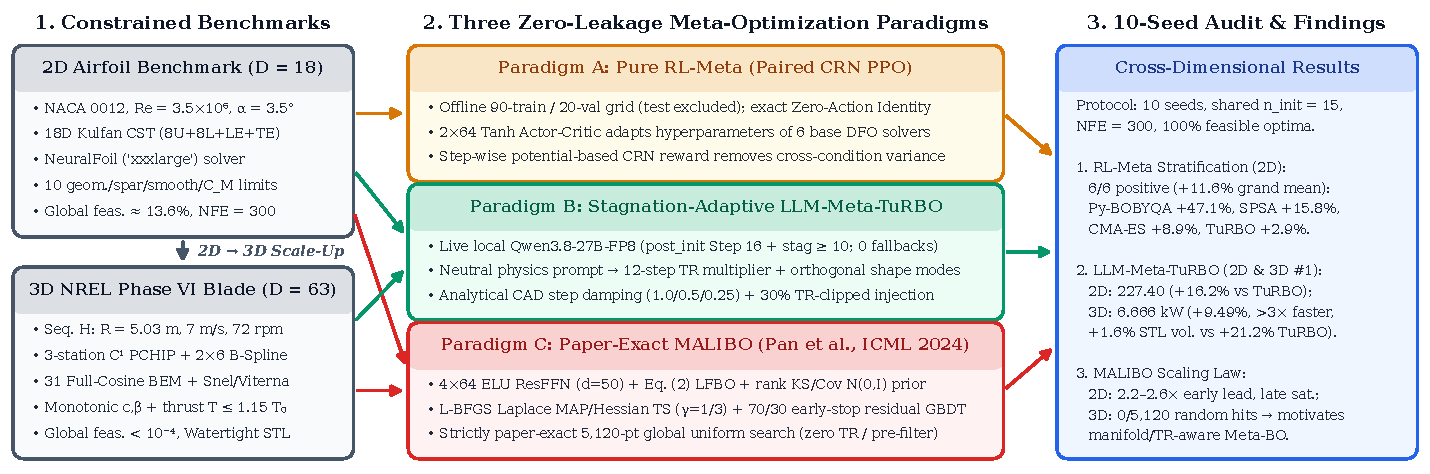
\includegraphics[width=0.92\textwidth]{figures/fig1_framework.pdf}
\vspace{-2mm}
\caption{Unified cross-dimensional meta-optimization architecture bridging 2D constrained airfoil design ($D=18$) and 3D NREL Phase VI wind turbine blade design ($D=63$) across Pure RL-Meta (Paired CRN PPO), Stagnation-Adaptive LLM-Meta-TuRBO, and Paper-Exact MALIBO.}
\label{fig:framework}
\end{figure*}

\jsubsection{Pure RL-Meta with Paired CRN Control-Variate PPO}
Dynamic hyperparameter control of a base DFO solver is modeled as a finite-horizon MDP $(\mathcal{S}, \mathcal{A}, r, \pi_\phi)$. At decision epoch $k$, the solver exposes a compact dimensionless state $\mathbf{s}_k \in \mathcal{S}$ comprising six shared progress/performance features---budget fraction $t/300$, normalized $\log_{10} Re$, normalized $\alpha$, cumulative relative gain, recent windowed gain, and stagnation ratio---augmented with 3--5 solver-specific internal diagnostics (Table~\ref{tab:rl_mdp}). A continuous Actor-Critic MLP ($2 \times 64$ \texttt{Tanh} hidden layers, orthogonal initialization) outputs bounded actions $\mathbf{a}_k \in [-1, 1]^{d_a}$ mapped multiplicatively or additively onto the base solver's hyperparameters.

\begin{table*}[t]
\centering
\caption{Six derivative-free base solvers, authoritative Vanilla defaults, and zero-action-identical RL-Meta MDP specifications (2D, $D=18$).}
\label{tab:rl_mdp}
\vspace{1mm}
\scriptsize
\setlength{\tabcolsep}{4.2pt}
\begin{tabular}{@{}l c l l l@{}}
\toprule
Optimizer & $d_s / d_a$ & Vanilla Default Schedule & Solver-Specific State Features & Action Modulation ($\mathbf{a}=\mathbf{0} \Rightarrow \text{Vanilla}$) \\
\midrule
Py-BOBYQA & 10 / 1 & Powell (2009): $\rho_{\text{beg}}=0.10, \rho_{\text{end}}=10^{-4}$ & $\log(\Delta/\rho_{\text{beg}}), \log(\rho/\rho_{\text{end}}), f_{\text{feas}}, \log\|\mathbf{g}\|$ & $\Delta \leftarrow \text{clip}(\Delta \cdot e^{0.35 a_1},\, \rho,\, \max(4\rho_{\text{beg}}, \Delta))$ \\
SPSA & 10 / 3 & Spall (1998): $c_{\text{rel}}=0.03, \text{clip}=0.10$ & $\log_{10} a_{\text{van}}, f_{\text{feas}}, r_{\text{clip}}, \text{med}|\Delta x/\text{span}|$ & $(a_k, c_k, \text{clip}_k)$ scaled by $(e^{1.2 a_1}, e^{0.8 a_2}, e^{1.4 a_3})$ \\
CMA-ES & 9 / 1 & Hansen (2006): $\sigma_0=0.05, \lambda=12$ & $\log(\sigma/\sigma_0), \|\mathbf{p}_\sigma\|/\chi_D, \log_{10}\kappa(\mathbf{C})$ & $\sigma \leftarrow \text{clip}(\sigma \cdot e^{0.40 a_1},\, 10^{-4}, 0.25)$ \\
DE & 11 / 2 & Storn--Price (1997): $F=0.7, CR=0.8, N_p=12$ & $CR, F, f_{\text{feas}}, \sigma_{\text{fit}}, \text{div}_{\text{pop}}$ & $F \in [0.35, 1.05]\,(e^{0.35 a_1}),\; CR \in [0.50, 0.95]$ \\
TuRBO & 10 / 2 & Eriksson et al.\ (2019): $L_0=0.8, \tau_s=3, \tau_f=4$ & $\log(L/L_0), n_{\text{succ}}, n_{\text{fail}}, \bar{\sigma}_{\text{GP}}$ & $L = \text{clip}(L_{\text{base}} e^{0.30 a_1}),\; \tau_{\text{TS}} \in [0.70, 1.40]$ \\
PSO & 11 / 3 & Clerc--Kennedy (2002): $w=0.7298, c_{1,2}=1.496$ & $w, c_1, c_2, \text{div}_{\text{sw}}, f_{\text{feas}}$ & $w \in [0.58, 0.83],\; c_{1,2} \in [1.15, 1.85]$ \\
\bottomrule
\end{tabular}
\end{table*}

Two strict methodological safeguards guarantee zero hidden bias:
\begin{enumerate}
\setlength{\itemsep}{1pt}\setlength{\parskip}{0pt}\setlength{\topsep}{2pt}
\item \emph{Zero-Action Identity Verification:} For all six solvers, setting $\mathbf{a}_k \equiv \mathbf{0}$ reproduces the untouched Vanilla trajectory bit-for-bit ($\max|J_{\text{meta}}(\mathbf{0}) - J_{\text{van}}| = 0.00 \times 10^0$), ruling out hidden architectural privileges.
\item \emph{Paired CRN Control-Variate Reward and 90/20 Validation:} Training operates strictly on a $10 \times 11 = 110$ offline grid ($Re \in \{1,\dots,10\}\times 10^6$, $\alpha \in \{0,\dots,10\}^\circ$), partitioned into 90 training and 20 internal-validation conditions that strictly exclude $(3.5\times 10^6, 3.5^\circ)$. Each training episode executes the meta-policy and Vanilla baseline under identical $(Re, \alpha, \text{seed})$, normalizing rewards by $S = \max(J_{\text{van}}^{\text{best}} - J_0, 15)$. For long-horizon solvers (\texttt{SPSA} $T=148$, \texttt{TuRBO} $T=285$), where GAE discounting ($\gamma=0.99, \lambda_{\text{GAE}}=0.95$) attenuates terminal credit, we apply step-wise potential-based trajectory shaping (Ng et al., 1999):
\be
r_k = \frac{2.5}{S}\bigl(\Delta J_{\text{meta},k} - 0.8\,\Delta J_{\text{van},k}\bigr) + \mathbb{I}[k=T]\,\text{clip}\!\left(\frac{J_{\text{meta}}^{\text{best}} - J_{\text{van}}^{\text{best}}}{S}, -1.5, 1.5\right).
\label{eq:crn_reward}
\ee
Policies are updated with clipped PPO ($\epsilon=0.20$, linear LR decay $3\times 10^{-4} \to 5\times 10^{-5}$, entropy weight $0.005$, 450 episodes for SPSA/Py-BOBYQA/DE/PSO/CMA-ES and 300 episodes for TuRBO), retaining the best checkpoint on the 20 internal validation tasks (starting from the 0\% identity baseline).
\end{enumerate}

\jsubsection{Paper-Exact Likelihood-Free Bayesian Meta-Learning (MALIBO)}
To preserve an exact scientific baseline for high-dimensional constrained ASO, we implement MALIBO strictly following Pan et al.\ (2024) without adding trust regions, coordinate sparsity masks, or free geometric pre-filters. Given $T$ offline meta-tasks $\mathcal{D}^{\text{meta}} = \{\mathcal{D}^t\}_{t=1}^T$ (with $y_i^t = -J(\mathbf{x}_i^t)$ cast as minimization and quantile threshold $\tau_t = \Phi_t^{-1}(\gamma)$ at fixed $\gamma = 1/3$), MALIBO models the likelihood-free Expected Improvement classifier $C_t(\mathbf{x}) = \sigma\bigl(m(\bm{\Phi}) + \mathbf{z}_t^\top \bm{\Phi}\bigr)$, where $\bm{\Phi} = \phi(\mathbf{x}) \in \mathbb{R}^{50}$ is a shared 4-layer, 64-unit ELU Residual Feedforward Network (ResFFN), $m(\cdot)$ is a task-agnostic mean prediction head, and $\mathbf{z}_t \in \mathbb{R}^{50}$ is a task-specific latent embedding. Meta-training minimizes the LFBO weighted classification objective (Song et al., 2022) plus a tractable Gaussian prior regularizer (Saseendran et al., 2021):
\be
\mathcal{L}^{\text{meta}}\!\left(\bm{\omega}, \{\mathbf{z}_t\}_{t=1}^T\right) = \frac{1}{T}\sum_{t=1}^T \mathcal{L}^{\text{LFBO}}(\bm{\omega}, \mathbf{z}_t; \mathcal{D}^t, \tau_t) + \lambda\,\mathcal{R}\!\left(\{\mathbf{z}_t\}_{t=1}^T; \mathcal{N}(\mathbf{0}, \mathbf{I})\right),
\label{eq:malibo_meta}
\ee
with $\lambda = 0.1$ and the exact LFBO utility loss:
\be
\mathcal{L}^{\text{LFBO}} = -\mathbb{E}_{(\mathbf{x},y)\sim \mathcal{D}^t}\!\left[\max(\tau_t - y, 0)\ln C_t(\mathbf{x}) + \ln\bigl(1 - C_t(\mathbf{x})\bigr)\right],
\label{eq:lfbo_loss}
\ee
evaluated via numerically stable softplus logits, while $\mathcal{R}$ combines rank-ordered marginal Kolmogorov--Smirnov (KS) CDF matching and Frobenius covariance alignment ($\|\mathbf{I} - \text{Cov}(\{\mathbf{z}_t\})\|_F^2$) with Monte-Carlo calibrated weights $(\lambda_{\text{KS}}, \lambda_{\text{Cov}})$ from Pan et al.\ (2024, Appendix C).

During online target-task optimization, the frozen ResFFN adapts to $\mathcal{D}_N$ via L-BFGS (\texttt{strong\_wolfe}) to obtain $\mathbf{z}_{\text{MAP}} = \arg\min_{\mathbf{z}} \bigl[\frac{1}{2}\mathbf{z}^\top\mathbf{z} + \sum_{n=1}^N \mathcal{L}_n^{\text{LFBO}}(\mathbf{z})\bigr]$ and the Laplace posterior precision matrix:
\be
\bm{\Sigma}_N^{-1} = \mathbf{I} + \sum_{n=1}^N \bigl(k_n(\tau - y_n) + 1\bigr)\,\hat{k}_n(1 - \hat{k}_n)\,\bm{\Phi}_n\bm{\Phi}_n^\top.
\label{eq:laplace}
\ee
A Thompson sample $\hat{\mathbf{z}} \sim \mathcal{N}(\mathbf{z}_{\text{MAP}}, \bm{\Sigma}_N)$ forms the strong base estimator for an online residual GBDT classifier (70/30 random split early stopping):
\be
C_{\text{GB}}(\mathbf{x}; \hat{\mathbf{z}}) = \sigma\!\left(m(\phi(\mathbf{x})) + \hat{\mathbf{z}}^\top\phi(\mathbf{x}) + \sum_{i=1}^{M} r_i(\mathbf{x})\right).
\label{eq:malibo_gb}
\ee
Following Appendix G of Pan et al.\ (2024), the next query $\mathbf{x}_{N+1} = \arg\max_{\mathbf{x} \in \mathcal{C}} C_{\text{GB}}(\mathbf{x}; \hat{\mathbf{z}})$ is selected by uniform global random search over $|\mathcal{C}| = 5,120$ points in $[0, 1]^D$. Offline meta-datasets strictly exclude all test points: 250 tasks (5 airfoils $\times$ 10 $Re \times$ 5 $\alpha$, 75,000 samples) in 2D (80/20 early-stopped Val Loss $= 0.2452$, $\text{std}(\mathbf{z}_t) = 0.9980$), and 100 multi-speed/RPM/pitch tasks (20,000 samples) in 3D (Val Loss $= 0.0272$, $\text{std}(\mathbf{z}_t) = 1.0057$).

\jsubsection{Zero-Leakage Stagnation-Adaptive LLM-Meta-TuRBO}
To inject domain aerodynamic reasoning into high-dimensional Bayesian optimization without compromising scientific integrity, we couple TuRBO-1 (Mat\'ern-5/2 GP surrogate with Cholesky Thompson sampling and native trust-region length $L_{\text{base}}$) with a live local LLM meta-controller served via SGLang (\texttt{Qwen/Qwen3.8-27B-FP8}, \texttt{enable\_thinking=False}, temperature $0.6$). Five strict design principles govern the controller:
\begin{enumerate}
\setlength{\itemsep}{1pt}\setlength{\parskip}{0pt}\setlength{\topsep}{2pt}
\item \emph{Zero Fallback and Neutral Prompts:} Any API or JSON parsing failure raises a hard exception (zero silent heuristic fallbacks). Prompts supply only physical state summaries (current $C_L, C_D, C_M, t_{\max}$ in 2D; power, $C_p$, thrust margin, and 3-station $c, \beta, t/c$ in 3D) and general aerodynamic constraints, with zero numerical target hints.
\item \emph{Stagnation-Adaptive Triggering:} After the shared $n_{\text{init}}=15$ initialization, the LLM executes a single \texttt{post\_init} diagnostic at Step 16; thereafter, interventions trigger strictly upon genuine stagnation ($\ge 10$ consecutive non-improving evaluations, minimum spacing 18 steps, capped at Step $\le 180$), yielding only $5.1$ calls/seed in 2D and $7.2$ calls/seed in 3D.
\item \emph{Temporary Trust-Region Modulation:} Each LLM response outputs a temporary trust-region multiplier $\kappa_L \in [0.70, 1.50]$ applied multiplicatively as $L = \text{clip}(L_{\text{base}}\cdot\kappa_L, L_{\min}, L_{\max})$ that decays cleanly to $1.0$ after 12 evaluations without corrupting TuRBO's native success/failure state machine, alongside coordinate perturbation probability $p_{\text{perturb}}$ and Thompson sampling temperature $\tau_{\text{TS}}$.
\item \emph{Smooth Orthogonal Physical Shape Modes:} Optionally, the LLM specifies a macroscopic deformation vector along smooth physical basis functions. In 2D, four strictly symmetric channels perturb Bernstein coordinates $u_i = (i+0.5)/8$: mid-chord camber $\sin(\pi u)$, aft loading $u^2\sin(\pi u)$, symmetric thickness $\pm 0.5\sin(\pi u)$, and leading-edge weight $w_{\text{LE}}$. In 3D, twelve zone-aligned channels adjust camber, thickness, chord, and twist across Root, Mid, and Tip stations using smooth sine envelopes (with mildly asymmetric textbook wind-turbine schema ranges such as $\Delta\beta_{\text{root}} \in [-4^\circ, +2^\circ]$ and camber $\in [-0.04, +0.06]$ transparently disclosed).
\item \emph{Analytical Step Damping and 30\% TR-Clipped Injection:} Proposed macro shifts undergo zero-NFE analytical geometric feasibility backtracking ($s \in \{1.0, 0.5, 0.25\}$) before consuming one evaluation; if feasible, its unit direction $\hat{\mathbf{d}}_u$ guides $30\%$ of TuRBO's local Thompson candidates (strictly clipped to the current trust region $[\mathbf{x}_{\text{best}} \pm L/2]$) over the next 15 steps, while $70\%$ retain standard isotropic TuRBO exploration.
\end{enumerate}

%======================================================================
\jsection{2D Airfoil Optimization Results}
%======================================================================
All 2D evaluations use 10 independent random seeds (\texttt{42, 123, 256, 777, 1024, 2024, 3407, 5555, 8888, 9999}), strict budget $\text{NFE}=300$, and identical $n_{\text{init}}=15$ initialization for all four TuRBO/MALIBO paradigms (baseline NACA 0012 plus 14 symmetric $\pm 0.03$ perturbations, yielding identical Step-15 mean $72.47 \pm 2.24$). Following standard reporting across all experimental logs, dispersion is reported as population standard deviation ($\text{ddof}=0$), and pairwise significance is assessed via two-sided paired $t$-tests ($p_t$), Wilcoxon signed-rank tests ($p_w$), and paired Cohen's $d$. Every single optimum across all 140 independent 2D runs satisfies 100\% of the ten industrial constraints.

\jsubsection{Pure RL-Meta Across Six Classic Derivative-Free Solvers}
Table~\ref{tab:2d_rlmeta} and Figure~\ref{fig:2d_rlmeta} summarize the 10-seed comparison between untouched Vanilla defaults and zero-action-identical RL-Meta policies across all six base optimizers. RL-Meta achieves a \textbf{6/6 strictly positive improvement}, lifting the six-solver grand mean from $180.87$ to $201.85$ ($+20.99$, $+11.6\%$) with zero degradation on any algorithm.

\begin{table*}[t]
\centering
\caption{Pure RL-Meta vs.\ Vanilla benchmark across six derivative-free optimizers on 2D NACA 0012 ($Re=3.5\times 10^6, \alpha=3.5^\circ$, 10 seeds, $\text{NFE}=300$, SD with $\text{ddof}=0$). All six solvers satisfy exact zero-action identity ($\text{diff}=0.00$) and achieve $10/10$ feasibility.}
\label{tab:2d_rlmeta}
\vspace{0.5mm}
\scriptsize
\setlength{\tabcolsep}{2.7pt}
\begin{tabular}{@{}l c c c c c c c c c@{}}
\toprule
Optimizer & Vanilla Mean $\pm$ SD & Van.\ Med.\ [Min, Max] & RL-Meta Mean $\pm$ SD & Meta Med.\ [Min, Max] & $\Delta$ (Rel.\ \%) & Win & $t$ ($p_t$) & $p_w$ & $d$ \\
\midrule
\textbf{Py-BOBYQA} & $136.19 \pm 30.95$ & 123.31 [98.6, 180.5] & $\mathbf{200.33 \pm 22.66}$ & \textbf{206.44} [159.7, 231.4] & $\mathbf{+64.13\ (+47.1\%)}$ & \textbf{10/10} & $+8.898$ ($<10^{-4}$) & \textbf{0.0020} & $\mathbf{+2.81}$ \\
\textbf{SPSA} & $186.93 \pm 21.08$ & 187.57 [149.5, 216.9] & $\mathbf{216.45 \pm 16.43}$ & \textbf{222.39} [174.2, 232.2] & $\mathbf{+29.52\ (+15.8\%)}$ & \textbf{8/10} & $+2.981$ (\textbf{0.0154}) & \textbf{0.0195} & $\mathbf{+0.94}$ \\
\textbf{CMA-ES} & $189.19 \pm 11.69$ & 188.23 [165.6, 210.6] & $\mathbf{206.10 \pm 12.08}$ & \textbf{207.94} [183.5, 224.4] & $\mathbf{+16.90\ (+8.9\%)}$ & \textbf{9/10} & $+3.730$ (\textbf{0.0047}) & \textbf{0.0059} & $\mathbf{+1.18}$ \\
DE & $181.90 \pm 13.87$ & 183.09 [157.7, 206.9] & $191.25 \pm 25.64$ & 192.63 [156.7, 233.1] & $+9.34\ (+5.1\%)$ & 5/10 & $+1.023$ (0.3329) & 0.4316 & $+0.32$ \\
TuRBO & $195.73 \pm 12.32$ & 198.97 [164.2, 207.6] & $201.46 \pm 13.09$ & 199.58 [182.6, 232.6] & $+5.74\ (+2.9\%)$ & 7/10 & $+1.079$ (0.3089) & 0.2324 & $+0.34$ \\
PSO & $195.24 \pm 13.52$ & 201.44 [167.4, 208.8] & $195.54 \pm 23.46$ & 202.81 [156.9, 236.3] & $+0.29\ (+0.2\%)$ & 6/10 & $+0.052$ (0.9594) & 0.9219 & $+0.02$ \\
\midrule
\textbf{Grand Mean} & $180.87$ & -- & $\mathbf{201.85}$ & -- & $\mathbf{+20.99\ (+11.6\%)}$ & \textbf{6/6} & -- & -- & -- \\
\bottomrule
\end{tabular}
\end{table*}

\begin{figure*}[t]
\centering
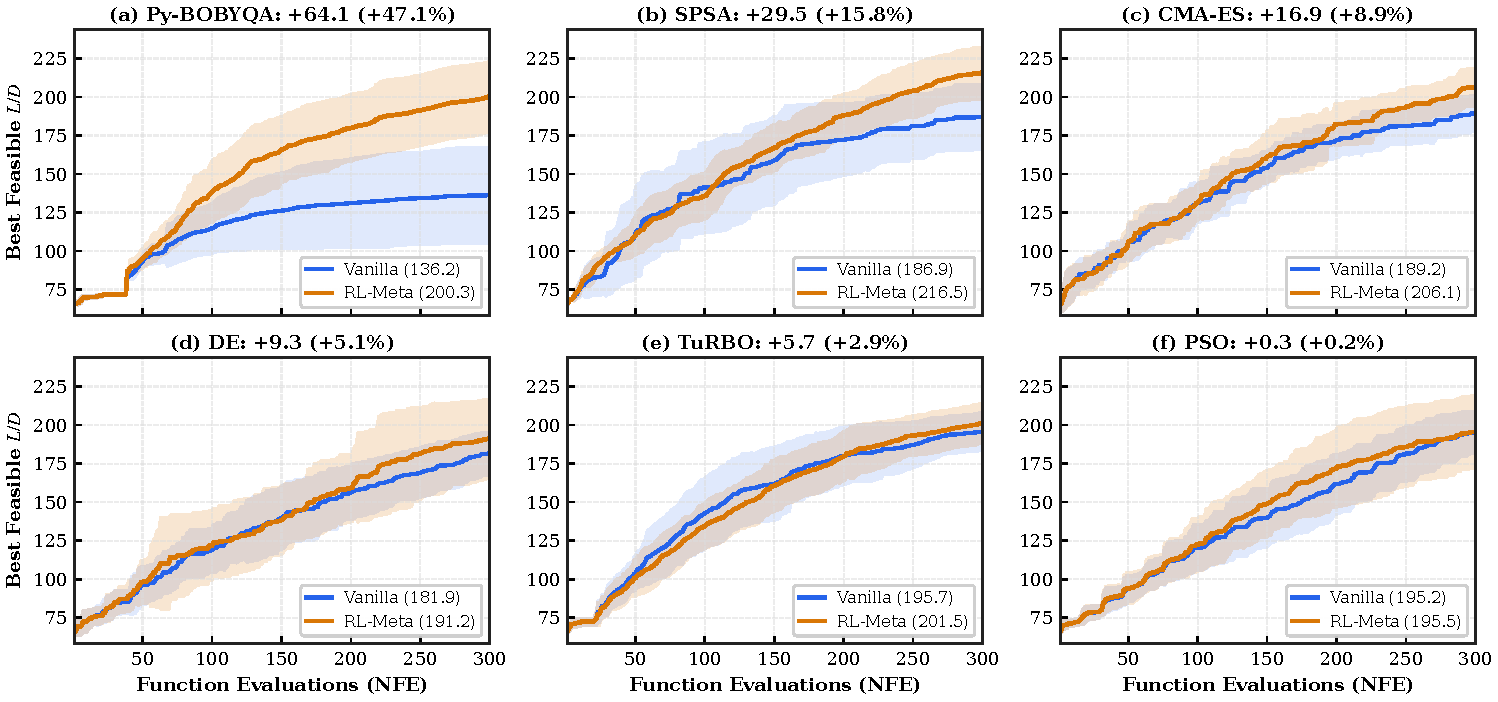
\includegraphics[width=0.84\textwidth]{figures/fig2_2d_rlmeta_convergence.pdf}
\vspace{-2mm}
\caption{Mean $\pm$ SD convergence trajectories across 10 seeds comparing Vanilla defaults against zero-action-identical Pure RL-Meta on six derivative-free optimizers, ordered by relative gain to illustrate the hyperparameter-sensitivity stratification.}
\label{fig:2d_rlmeta}
\end{figure*}

More importantly, the results expose a clean, textbook \emph{hyperparameter-sensitivity stratification} governed by each base solver's intrinsic adaptability:
\begin{itemize}
\setlength{\itemsep}{1.5pt}\setlength{\parskip}{0pt}\setlength{\topsep}{2pt}
\item \emph{Rigid / Hyperparameter-Sensitive Classical Solvers ($>15\%$ significant gain):} Vanilla Py-BOBYQA suffers premature trust-region contraction around non-smooth constraint boundaries, stalling at $136.19 \pm 30.95$; RL-Meta dynamically sustains $\Delta$ to reach $200.33 \pm 22.66$ ($+47.1\%$, $10/10$ wins, $p_t < 10^{-4}$, $d = +2.81$). Likewise, exposing SPSA's step-clipping trust bound alongside $(a_k, c_k)$ under step-wise CRN potential shaping allows PPO to decouple gradient progress ($\text{scale}_a \approx 0.80\text{--}0.87\times$) from constraint-cliff overshoot ($\text{scale}_{\text{clip}}: 0.34\times \to 0.27\times$), boosting online evaluation feasibility from $75.9\%$ to $88.7\%$, reducing cross-seed SD by $22\%$, and raising RL-Meta-SPSA to the highest RL-Meta score of $216.45 \pm 16.43$ ($+15.8\%$, $p_t = 0.0154$, median $222.39$, peak $232.24$).
\item \emph{Self-Adaptive Evolutionary Solvers ($5\%\text{--}9\%$ gain):} CMA-ES improves significantly by $+16.90$ ($+8.9\%$, $9/10$ wins, $p_t = 0.0047$, $d = +1.18$) via learned step-size modulation; DE gains $+9.34$ ($+5.1\%$).
\item \emph{Sophisticated Surrogate / Tightly Calibrated Solvers ($0.2\%\text{--}3\%$ non-harmful gain):} TuRBO already incorporates GP modeling and adaptive trust-region logic, while Clerc--Kennedy PSO sits near its theoretical stability manifold; pure black-box PPO accordingly delivers modest, strictly safe gains ($+2.9\%$ on TuRBO with worst seed lifted from $164.2$ to $182.6$; $+0.2\%$ on PSO).
\end{itemize}
This diminishing-returns phenomenon on already sophisticated surrogate solvers directly motivates pairing TuRBO with higher-level prior knowledge via MALIBO or domain-aware LLM meta-control.

\jsubsection{Four-Paradigm Comparison on 2D Airfoil}
Table~\ref{tab:2d_paradigms} and Figures~\ref{fig:2d_paradigms}--\ref{fig:2d_shapes} compare Vanilla-TuRBO, RL-Meta-TuRBO, LLM-Meta-TuRBO, and Paper-Exact MALIBO under identical initialization and budget.

\begin{table*}[t]
\centering
\caption{Four-paradigm benchmark on 2D NACA 0012 ($D=18$, 10 seeds, $\text{NFE}=300$, shared $n_{\text{init}}=15$ mean $72.47 \pm 2.24$). NFE columns list the earliest step where the 10-seed mean curve reaches the given $L/D$ threshold (`--' denotes not reached within 300 NFE).}
\label{tab:2d_paradigms}
\vspace{1mm}
\scriptsize
\setlength{\tabcolsep}{3.6pt}
\begin{tabular}{@{}l c c c c c c c c c@{}}
\toprule
\multirow{2}{*}{Method} & Final $L/D$ & Med.\ [Min, Max] & $\Delta$ vs.\ TuRBO & \multicolumn{4}{c}{NFE to Reach $L/D \ge$} & Median Airfoil & Time / \\
\cmidrule(lr){5-8}
 & (Mean $\pm$ SD) & ($L/D$) & ($p_t$ / $d$) & 100 & 120 & 160 & 200 & ($C_L / C_D / C_M / t_{\max}$) & Seed \\
\midrule
Vanilla-TuRBO & $195.73 \pm 12.32$ & 198.97 [164.2, 207.6] & Baseline & 46 & 69 & 140 & -- & $0.896 / .00448 / -.097 / 11.5\%$ & $\approx 1.0\,\text{s}$ \\
RL-Meta-TuRBO & $201.46 \pm 13.09$ & 199.58 [182.6, 232.6] & $+5.74$ (.309 / .34) & 49 & 80 & 148 & 293 & $0.911 / .00451 / -.106 / 13.6\%$ & $\approx 1.0\,\text{s}$ \\
\textbf{LLM-Meta-TuRBO} & $\mathbf{227.40 \pm 13.41}$ & \textbf{225.10} [200.8, 247.1] & $\mathbf{+31.67}$ (\textbf{.0018} / \textbf{1.38}) & \textbf{16} & \textbf{18} & \textbf{40} & \textbf{120} & $0.960 / .00424 / -.134 / 13.0\%$ & $39.4\,\text{s}$ \\
MALIBO (Paper-Exact) & $179.81 \pm 9.29$ & 180.00 [166.7, 192.9] & $-15.92$ (.0126 / $-.98$) & 21 & 31 & 114 & -- & $0.839 / .00463 / -.108 / 15.6\%$ & $66.6\,\text{s}$ \\
\bottomrule
\end{tabular}
\end{table*}

\begin{figure*}[t]
\centering
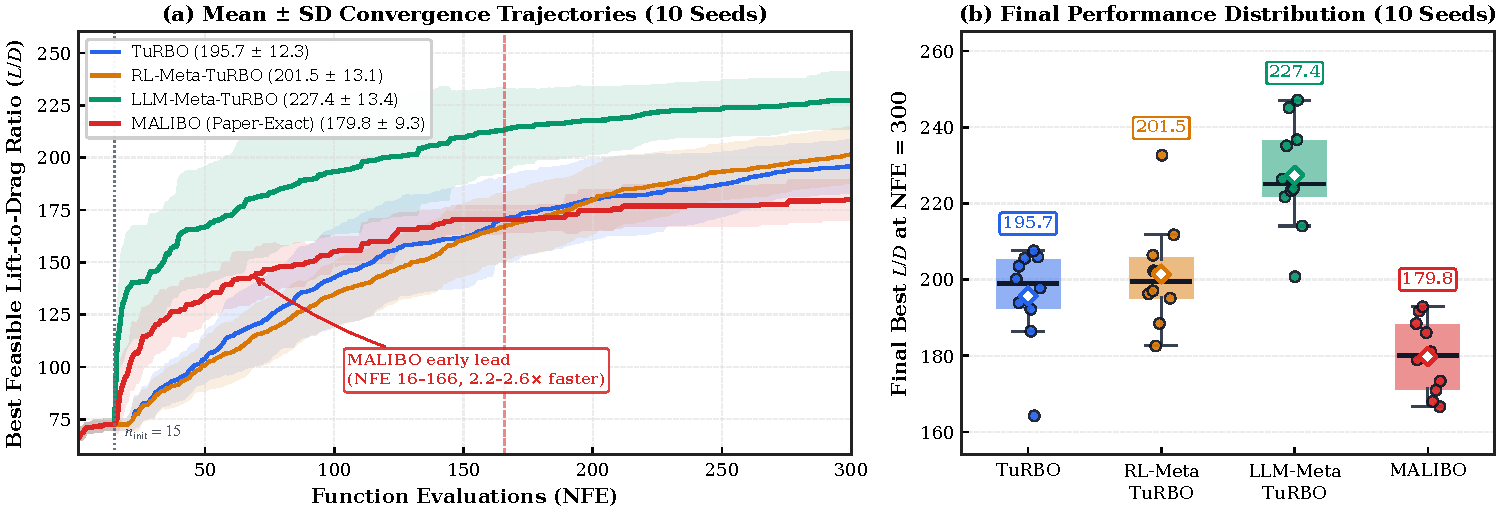
\includegraphics[width=0.86\textwidth]{figures/fig3_2d_paradigms_perf.pdf}
\vspace{-2mm}
\caption{Four-paradigm comparison on the 2D constrained airfoil benchmark ($D=18$, 10 seeds): (a) Mean $\pm$ SD convergence trajectories highlighting MALIBO's early transfer speedup (NFE 16--166) and LLM-Meta-TuRBO's full-horizon dominance; (b) final $L/D$ distributions with individual seeds and mean diamonds.}
\label{fig:2d_paradigms}
\end{figure*}

Two distinct and complementary physical mechanisms emerge:
\begin{enumerate}
\setlength{\itemsep}{1.0pt}\setlength{\parskip}{0pt}\setlength{\topsep}{2pt}
\item \emph{Zero-Leakage LLM-Meta-TuRBO Dominates Across the Full Horizon:} Without any numerical answers in its prompt, \texttt{Qwen3.8-27B-FP8} triggers an average of only $5.1$ calls/seed (range 3--7, $39.4\,\text{s}$ wall time), achieving a $56.9\%$ immediate improvement rate on its macroscopic directional steps. It reaches $L/D \ge 160$ in 40 evaluations ($3.50\times\text{--}3.70\times$ faster than Vanilla/RL-Meta-TuRBO) and $L/D \ge 200$ in 120 evaluations ($2.44\times$ faster than RL-Meta-TuRBO's 293 NFE). At NFE 300, it achieves $227.40 \pm 13.41$ (peak $247.11$), decisively outperforming Vanilla-TuRBO ($9/10$ wins, $p_t = 0.0018, p_w = 0.0039, d = +1.38$), RL-Meta-TuRBO ($+25.94$, $9/10$ wins, $p_t = 0.0114, p_w = 0.0195, d = +1.00$), and MALIBO ($10/10$ wins, $p_t < 10^{-5}, d = +3.16$). As shown in Fig.~\ref{fig:2d_shapes}, the LLM-guided median airfoil smoothly increases mid-to-aft camber while maintaining $t_{\max} = 13.02\%$ and respecting $C_M = -0.1341 \ge -0.15$, attaining both highest lift ($C_L = 0.9599$) and lowest drag ($C_D = 0.00424$).
\item \emph{Paper-Exact MALIBO Exhibits a Sharp Early-Transfer vs.\ Late-Saturation Trade-Off:} Leveraging its 250-task meta-learned ResFFN prior, MALIBO immediately accelerates after initialization, reaching $L/D \ge 100$ in 21 NFE ($2.19\times$ faster than TuRBO, $2.33\times$ faster than RL-Meta-TuRBO) and $L/D \ge 120$ in 31 NFE ($2.23\times\text{--}2.58\times$ speedup). MALIBO strictly leads Vanilla-TuRBO across NFE 16--166 and RL-Meta-TuRBO across NFE 16--175 while maintaining the lowest cross-seed variance ($\text{SD}=6.64$ at NFE 100, $29\%$ of TuRBO's SD; final $\text{SD}=9.29$). Beyond NFE 150, however, global 5,120-point uniform acquisition sampling in $[0,1]^{18}$ cannot contract locally around narrow high-$L/D$ ridges near active constraints, causing exploitation to saturate at $179.81 \pm 9.29$. An independent held-out sanity check on NACA 2412 ($Re = 2.5\times 10^6, \alpha = 5.0^\circ$, 100 NFE) confirms the exact same pattern: MALIBO dominates TuRBO through Step 90 before TuRBO edges ahead at Step 100 ($173.46$ vs.\ $170.45$, from baseline $114.02$).
\end{enumerate}

\begin{figure}[htb]
\centering
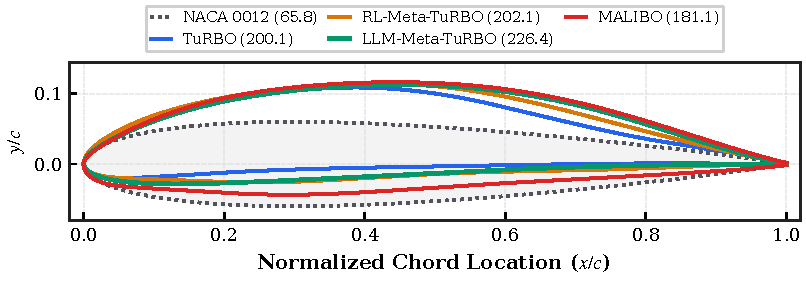
\includegraphics[width=0.95\linewidth]{figures/fig4_2d_airfoil_shapes.pdf}
\vspace{-2mm}
\caption{Representative median optimized 2D airfoil profiles ($Re=3.5\times 10^6, \alpha=3.5^\circ$, $\text{NFE}=300$) compared against baseline NACA 0012.}
\label{fig:2d_shapes}
\end{figure}

%======================================================================
\jsection{3D Wind Turbine Blade Optimization Results}
%======================================================================
We next transition to the 3D NREL Phase VI wind turbine blade ($D=63$, 31 full-cosine BEM sections, 10 seeds, $\text{NFE}=300$, shared $n_{\text{init}}=15$ baseline plus 14 symmetric $\pm 0.04$ unit perturbations yielding Step-15 mean $6.1773 \pm 0.0280\,\text{kW}$). Based on the 2D stratification finding that black-box PPO yields modest gains on TuRBO ($+2.9\%$), the computationally heavier 3D campaign focuses directly on TuRBO-1, LLM-Meta-TuRBO, and Paper-Exact MALIBO.

\jsubsection{Dimensionality Reduction Benefit ($D=114 \to D=63$)}
Before the 10-seed benchmark, we verified the geometric smoothness and search-space impact of our 3-station $C^1$ PCHIP + B-spline parameterization ($D=63$). In a 100-NFE diagnostic comparing discrete 3-station ($D=60$) and B-spline ($D=63$) models, both maintained near-zero chord curvature variance ($\text{Var}(\Delta^2 c) \le 4\times 10^{-6}$) and smooth twist variation ($\text{Var}(\Delta^2 \beta) \approx 0.029$, 1 inflection), with $D=63$ running $12.4\%$ faster ($175.3$ vs.\ $200.1\,\text{ms/step}$). Critically, condensing from an earlier 6-station piecewise-linear blade ($D=114$) to the 3-station $C^1$ PCHIP formulation ($D=63$) boosted 10-seed LLM-Meta-TuRBO gain from $+8.76\%$ ($6.6031 \pm 0.0358\,\text{kW}$) to $+9.49\%$ ($6.6664 \pm 0.0196\,\text{kW}$, $45\%$ lower SD) and TuRBO-1 from $+7.80\%$ ($6.5449 \pm 0.0638\,\text{kW}$) to $+8.27\%$ ($6.5920 \pm 0.0463\,\text{kW}$), while completely eliminating 3D side-view surface undulations.

\jsubsection{Ten-Seed 3D Benchmark and Statistical Significance}
Table~\ref{tab:3d_results} and Figure~\ref{fig:3d_perf} present the full 10-seed 3D results; all $30/30$ final designs achieve $100\%$ feasibility with zero constraint penalty (\texttt{max\_penalty} $= 0$) and axial thrust strictly bounded within $T_{\max} = 1.3954\,\text{kN}$.

\begin{table*}[t]
\centering
\caption{Ten-seed 3D NREL Phase VI wind turbine blade benchmark ($D=63$, 31 full-cosine BEM sections, $V_\infty=7.0\,\text{m/s}, 72\,\text{rpm}$, $\text{NFE}=300$). All 30 runs are 100\% feasible ($T \le 1.3954\,\text{kN}$). Peak STL volumes correspond to exported watertight 2-manifold meshes.}
\label{tab:3d_results}
\vspace{1mm}
\scriptsize
\setlength{\tabcolsep}{3.5pt}
\begin{tabular}{@{}l c c c c c c c c@{}}
\toprule
Method & Power Mean $\pm$ SD & Med.\ [Min, Max] & Torque $Q$ & $C_p$ & Gain vs. & Thrust $T$ & Peak $P$ / STL Vol. & Time / \\
 & (kW) & (kW) & (N$\cdot$m) & (--) & Base & (kN) & (kW / $\text{m}^3$ [$\Delta V$]) & Seed \\
\midrule
Baseline (Phase VI) & $6.0884$ & $6.0884$ & $807.50$ & $0.3647$ & $+0.00\%$ & $1.2134$ & $6.0884$ / $0.1446$ ($0.0\%$) & -- \\
TuRBO-1 & $6.5920 \pm 0.0463$ & 6.5717 [6.507, 6.653] & $874.29 \pm 6.14$ & $0.3949$ & $+8.27\%$ & $1.3938$ & $6.6526$ / $0.1753$ ($+21.2\%$) & $\mathbf{70.9\,\text{s}}$ \\
\textbf{LLM-Meta-TuRBO} & $\mathbf{6.6664 \pm 0.0196}$ & \textbf{6.6573} [6.646, 6.696] & $\mathbf{884.16 \pm 2.60}$ & $\mathbf{0.3994}$ & $\mathbf{+9.49\%}$ & $1.3948$ & $\mathbf{6.6955}$ / $\mathbf{0.1470}$ ($\mathbf{+1.6\%}$) & $157.9\,\text{s}$ \\
MALIBO (Paper-Exact) & $6.1773 \pm 0.0280$ & 6.1812 [6.125, 6.228] & $819.29 \pm 3.72$ & $0.3701$ & $+1.46\%$ & $1.2417$ & $6.2276$ / $0.1500$ ($+3.8\%$) & $111.0\,\text{s}$ \\
\bottomrule
\end{tabular}
\end{table*}

\begin{figure*}[t]
\centering
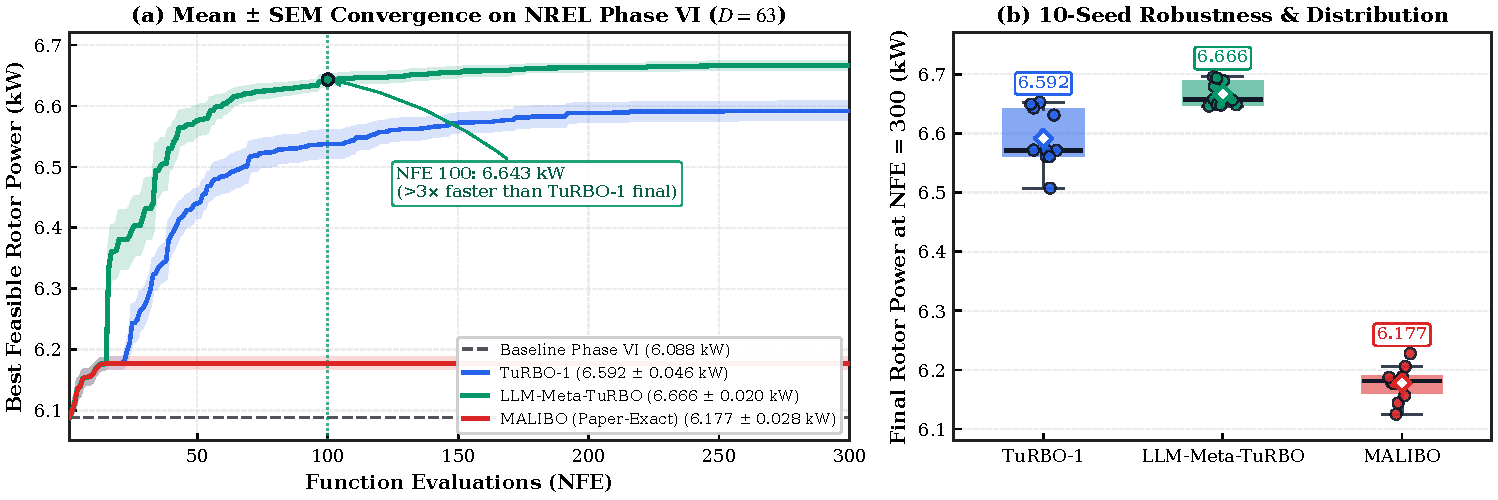
\includegraphics[width=0.86\textwidth]{figures/fig5_3d_blade_perf.pdf}
\vspace{-2mm}
\caption{Ten-seed optimization performance on the 3D NREL Phase VI rotor blade ($D=63$, $\text{NFE}=300$): (a) Mean $\pm$ SEM convergence trajectories demonstrating $>3\times$ sample-efficiency gain of LLM-Meta-TuRBO over TuRBO-1; (b) final power distribution across 10 seeds.}
\label{fig:3d_perf}
\end{figure*}

LLM-Meta-TuRBO establishes clear superiority across every performance and robustness metric. Invoking an average of $7.2$ live LLM calls/seed ($23.6\%$ immediate jump rate on macroscopic proposals), it achieves $6.6664 \pm 0.0196\,\text{kW}$ ($+9.49\%$ vs.\ baseline, $Q = 884.16\,\text{N}\cdot\text{m}$, $C_p = 0.3994$), significantly outperforming TuRBO-1 ($\Delta P = +0.0744\,\text{kW}$, $8/10$ wins, paired $t = 4.556$, $p_t = 0.00137$, Wilcoxon $p_w = 0.00977$, Cohen's $d = +1.44$). Remarkably, LLM-Meta-TuRBO reduces cross-seed SD by $58\%$ ($0.0196$ vs.\ $0.0463\,\text{kW}$)---its worst seed ($6.6463\,\text{kW}$) exceeds TuRBO-1's median ($6.5717\,\text{kW}$)---and reaches $6.6434\,\text{kW}$ by \textbf{NFE = 100}, surpassing TuRBO-1's full 300-NFE final mean ($6.5920\,\text{kW}$) for a \textbf{$>3\times$ sample-efficiency speedup} crucial when replacing BEM with expensive 3D CFD.

\jsubsection{3D Aerodynamic Mechanisms and Geometric Smoothness}
Figures~\ref{fig:3d_aero} and \ref{fig:3d_smooth} dissect the physical geometry of the peak-performing blades exported to watertight STLs:
\begin{itemize}
\setlength{\itemsep}{1.5pt}\setlength{\parskip}{0pt}\setlength{\topsep}{2pt}
\item \emph{Root Detwisting and Mid-Span AoA Matching:} Peak LLM-Meta-TuRBO (Seed 1024, $P = 6.6955\,\text{kW}$, $+9.97\%$, $Q = 888.0\,\text{N}\cdot\text{m}$, $C_p = 0.4011$---closely matching the $\approx 9.2\%\text{--}10\%$ Phase VI optimization headroom found in CFD by Kaya, 2019) smoothly reduces root twist from $20.04^\circ$ to $17.22^\circ$ while broadening root chord ($0.737 \to 0.803\,\text{m}$) and preserving structural thickness ($t/c = 20.2\%$). Across the primary torque-producing mid-span annulus ($r = 3.14\,\text{m}$), it enriches aft camber and moderately thins the section ($21.1\% \to 19.6\%$), shifting mid-span effective angle of attack from $8.3^\circ$ down into the optimal $6.0^\circ\text{--}7.5^\circ$ $C_L/C_D$ band (Fig.~\ref{fig:3d_aero}c,e).
\item \emph{Structural Lightweight Advantage:} Whereas blind local sampling in peak TuRBO-1 (Seed 42, $6.6526\,\text{kW}$) thickens the mid ($23.4\%$) and tip ($22.2\%$) stations, inflating total blade solid volume by $+21.2\%$ ($0.1753$ vs.\ $0.1446\,\text{m}^3$), LLM-Meta-TuRBO delivers higher power with only a \textbf{$+1.6\%$ solid volume increase} ($0.1470\,\text{m}^3$, surface area $4.49\,\text{m}^2$ vs.\ $4.65\,\text{m}^2$), lowering blade mass, centrifugal root loads, and material cost.
\item \emph{Zero Spanwise Undulations:} Orthographic top-view ($X$--$r$) and side-view ($Y$--$r$) envelopes in Fig.~\ref{fig:3d_smooth} verify smooth, monotonic, undulation-free lofting across all three control stations.
\end{itemize}

\begin{figure*}[t]
\centering
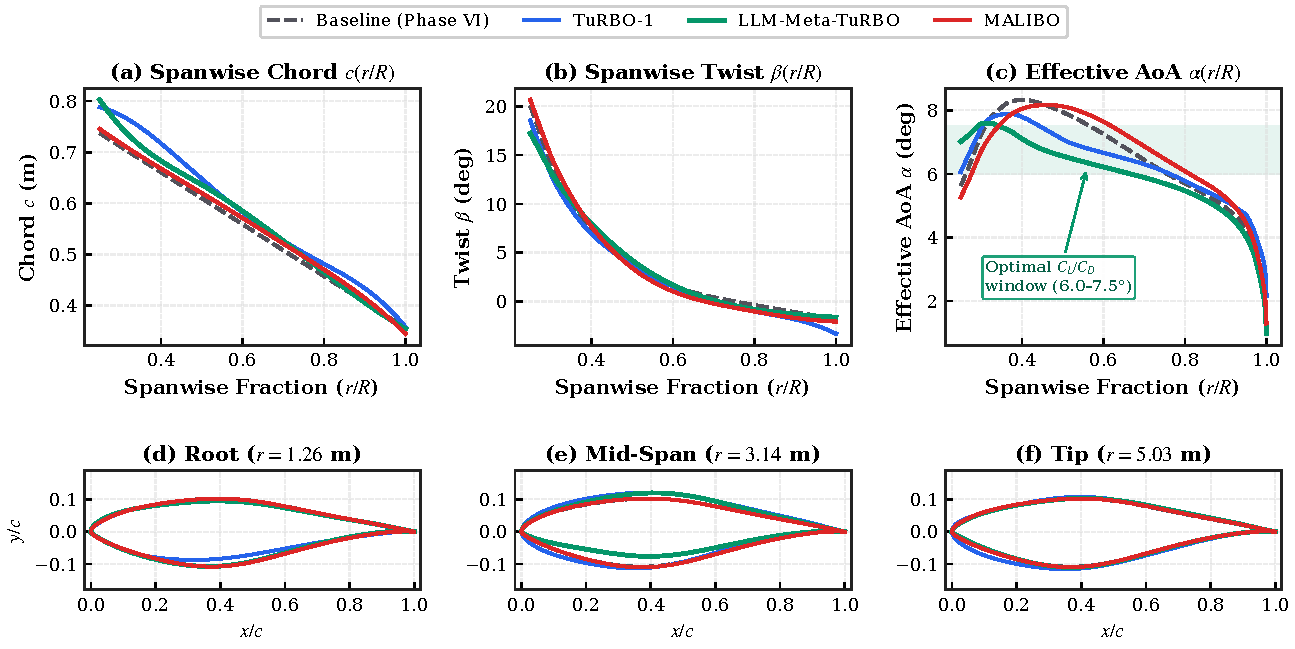
\includegraphics[width=0.83\textwidth]{figures/fig6_3d_blade_aero.pdf}
\vspace{-2mm}
\caption{Aerodynamic and geometric evolution of peak-performing 3D NREL Phase VI blades: (a) spanwise chord $c(r/R)$, (b) twist $\beta(r/R)$, (c) effective angle of attack $\alpha(r/R)$ entering the optimal $6.0^\circ\text{--}7.5^\circ$ window, and (d--f) cross-sectional airfoil profiles at Root, Mid-Span, and Tip control stations.}
\label{fig:3d_aero}
\end{figure*}

\begin{figure*}[t]
\centering
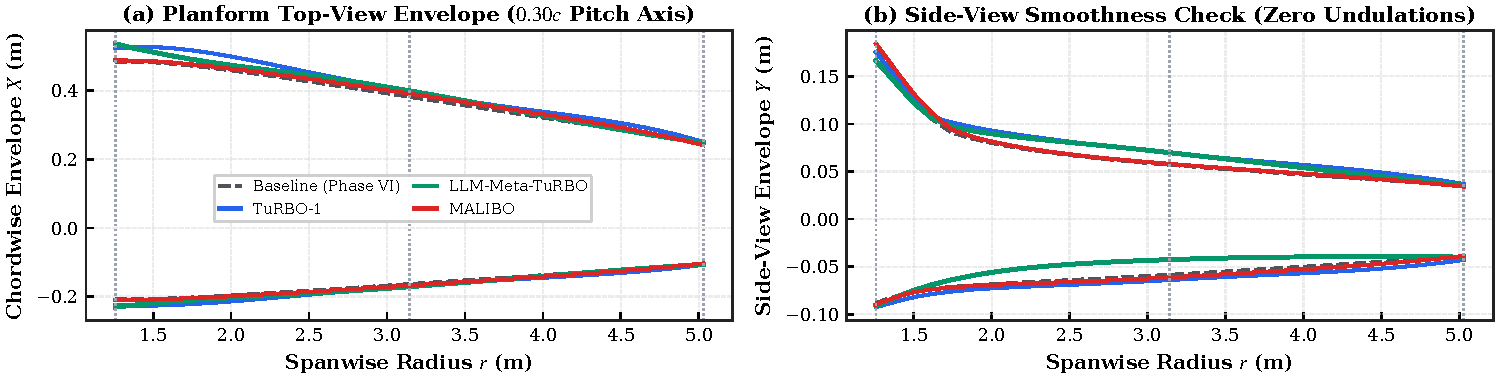
\includegraphics[width=0.84\textwidth]{figures/fig7_3d_blade_smoothness.pdf}
\vspace{-2mm}
\caption{Orthographic smoothness verification of 3D $C^1$ PCHIP lofted blades (vertical dotted lines denote Root, Mid, and Tip control stations): (a) planform top-view envelope aligned at $0.30c$ pitch axis; (b) side-view thickness envelope confirming zero spanwise undulations.}
\label{fig:3d_smooth}
\end{figure*}

\jsubsection{Cross-Dimensional Scaling Diagnosis of Paper-Exact MALIBO}
Contrasting MALIBO's behavior across 2D ($D=18$) and 3D ($D=63$) uncovers a fundamental structural limitation of global likelihood-free meta-BO under tight geometric constraints. In 3D, MALIBO's offline meta-training on 100 related wind/RPM/pitch tasks converges cleanly (early-stopped at epoch 435, $\text{Val Loss}=0.0272$, $\text{std}(\mathbf{z}_t)=1.0057$, $|\text{mean}|=0.0122$), confirming proper Bayesian prior alignment. Yet during online optimization on the target task, strictly adhering to Appendix G's 5,120-point global uniform search over $[0, 1]^{63}$ stalls completely at the shared Step-15 initialization gain ($6.1773 \pm 0.0280\,\text{kW}, +1.46\%$; Fig.~\ref{fig:3d_perf}a).

Diagnostic inspection explains why: enforcing simultaneous airfoil non-intersection, smoothness, spar thickness, spanwise chord/twist monotonicity, and curvature constraints shrinks the feasible manifold volume fraction from $\approx 13.6\%$ in 18D to $< 10^{-4}$ in 63D. Consequently, a global 5,120-point uniform draw hits \textbf{exactly $0 / 5,120$ geometrically feasible blades} (and only $39 / 5,120$ non-fatal shapes). Although the meta-learned classifier accurately recognizes that every sampled candidate lies outside the promising manifold---assigning strongly negative mean logits ($-3.41$ to $-4.20$) even to its top-10 candidates---an empty feasible candidate pool prevents any post-initialization improvement. Thus, MALIBO's failure in 63D is \emph{not} a meta-representation failure, but an exponential mismatch between global uniform acquisition search and thin high-dimensional feasible manifolds.

\jsubsection{Limitations and Future Work}
Three honest limitations frame our follow-up research: (i) aerodynamic evaluations currently employ high-accuracy physics-informed surrogates (\texttt{NeuralFoil xxxlarge} + corrected BEM) rather than live Navier--Stokes evaluations inside the loop; full 3D URANS CFD verification of our four exported watertight STLs (meshed to $y^+ \le 1$, first-cell height $y_1 \approx 2.5\times 10^{-5}\,\text{m}$ at $Re \approx 8\times 10^5$) is underway; (ii) feeding explicit closed-loop outcome summaries of prior LLM macro steps (e.g., whether an intervention saturated $C_M$ or thrust limits) into subsequent prompts can further increase immediate hit rates above $56.9\%$ (2D) and $23.6\%$ (3D); and (iii) the cross-dimensional MALIBO diagnosis directly motivates our ongoing journal development of \emph{Trust-Region and Manifold-Aware Likelihood-Free Meta-BO}, restricting MALIBO's acquisition optimization to adaptive local feasible subspaces.

%======================================================================
\jsection{Conclusions}
%======================================================================
This study presented a zero-leakage empirical investigation of reinforcement meta-learning (RL-Meta), stagnation-adaptive LLM meta-control (LLM-Meta-TuRBO), and paper-exact likelihood-free Bayesian meta-learning (MALIBO) across constrained 2D airfoil ($D=18$) and 3D NREL Phase VI wind turbine blade ($D=63$) shape optimization under a strict 300-evaluation budget. The principal conclusions are:
\begin{enumerate}
\setlength{\itemsep}{1.5pt}\setlength{\parskip}{0pt}\setlength{\topsep}{2pt}
\item \emph{Algorithm-Dependent RL-Meta Stratification:} Under exact zero-action identity and paired CRN PPO training, pure RL-Meta improves all six classical DFO solvers in 2D ($+11.6\%$ grand mean), yielding large statistically significant breakthroughs on hyperparameter-sensitive solvers (Py-BOBYQA $+47.1\%$, SPSA $+15.8\%$), steady gains on evolutionary methods (CMA-ES $+8.9\%$, DE $+5.1\%$), and strictly non-harmful gains on self-adaptive Bayesian/swarm baselines (TuRBO $+2.9\%$, PSO $+0.2\%$).
\item \emph{State-of-the-Art Performance of Stagnation-Adaptive LLM-Meta-TuRBO:} Combining neutral aerodynamic prompts, symmetric/smooth physical deformation bases, temporary trust-region multipliers, and stagnation-driven live LLM triggering achieves the highest accuracy and sample efficiency in both 2D ($L/D = 227.40 \pm 13.41$, $+16.2\%$ vs.\ TuRBO, $p=0.0018$) and 3D ($P = 6.6664 \pm 0.0196\,\text{kW}$, $+9.49\%$ vs.\ baseline, $p=0.0014$ vs.\ TuRBO-1, $>3\times$ speedup, $58\%$ lower variance, and $+9.97\%$ peak power gain at only $+1.6\%$ blade volume growth).
\item \emph{Cross-Dimensional Feasibility Law of Paper-Exact MALIBO:} Faithful likelihood-free meta-BO delivers strong $2.19\times\text{--}2.58\times$ early sample efficiency in 18D ($\approx 13.6\%$ global feasibility) before global sampling limits late exploitation, whereas in 63D ($<10^{-4}$ feasibility), global 5,120-point uniform acquisition search yields zero feasible hits despite accurate meta-learned latent priors, establishing a clear foundation for future trust-region and manifold-aware meta-BO algorithms.
\end{enumerate}

%======================================================================
\jsection{Acknowledgments}
%======================================================================
The authors acknowledge computational and research support from the College of Computing and Data Science, Nanyang Technological University, and the A*STAR Institute of Advanced Intelligence and Computing, Singapore.

%======================================================================
\section*{REFERENCES}
\par\vspace*{-0.5mm}

\isoperef{Buhl, ML (2005). \lq\lq A New Empirical Relationship between Thrust Coefficient and Induction Factor for the Turbulent Windmill State\rq\rq, {\it Technical Report NREL/TP-500-36834}, National Renewable Energy Laboratory, Golden, CO, USA.}

\isoperef{Cartis, C, Fiala, J, Marteau, B and Roberts, L (2019). \lq\lq Improving the Flexibility and Robustness of Model-Based Derivative-Free Optimization Solvers\rq\rq, {\it ACM Trans Mathematical Software}, Vol~45, No~3, pp~32:1--32:41.}

\isoperef{Clerc, M and Kennedy, J (2002). \lq\lq The Particle Swarm---Explosion, Stability, and Convergence in a Multidimensional Complex Space\rq\rq, {\it IEEE Trans Evolutionary Computation}, Vol~6, No~1, pp~58--73.}

\isoperef{Eriksson, D, Pearce, M, Gardner, J, Turner, RD and Poloczek, M (2019). \lq\lq Scalable Global Optimization via Local Bayesian Optimization\rq\rq, {\it Advances in Neural Information Processing Systems (NeurIPS)}, Vol~32, pp~5496--5507.}

\isoperef{Hand, MM, Simms, DA, Fingersh, LJ, Jager, DW, Cotrell, JR, Schreck, S and Larwood, SM (2001). \lq\lq Unsteady Aerodynamics Experiment Phase VI: Wind Tunnel Test Configurations and Available Data Campaigns\rq\rq, {\it Technical Report NREL/TP-500-29955}, National Renewable Energy Laboratory, Golden, CO, USA.}

\isoperef{Hansen, N (2006). \lq\lq The CMA Evolution Strategy: A Comparing Review\rq\rq, in {\it Towards a New Evolutionary Computation}, Springer, Berlin, pp~75--102.}

\isoperef{Kaya, M (2019). \lq\lq A CFD Based Application of Support Vector Regression to Determine the Optimum Smooth Twist for Wind Turbine Blades\rq\rq, {\it Sustainability}, Vol~11, No~16, 4502.}

\isoperef{Kulfan, BM (2008). \lq\lq Universal Parametric Geometry Representation Method\rq\rq, {\it J Aircraft}, Vol~45, No~1, pp~142--158.}

\isoperef{Liu, T, Astorga, N, Seedat, N and van der Schaar, M (2024). \lq\lq Large Language Models to Enhance Bayesian Optimization\rq\rq, {\it Proc Intl Conf Learning Representations (ICLR)}, Vienna, Austria.}

\isoperef{Martins, JRRA (2022). \lq\lq Aerodynamic Design Optimization: Challenges and Perspectives\rq\rq, {\it Computers \& Fluids}, Vol~239, 105391.}

\isoperef{Ng, AY, Harada, D and Russell, S (1999). \lq\lq Policy Invariance Under Reward Transformations: Theory and Application to Reward Shaping\rq\rq, {\it Proc 16th Intl Conf Machine Learning (ICML)}, San Francisco, CA, pp~278--287.}

\isoperef{Pan, J, Falkner, S, Berkenkamp, F and Vanschoren, J (2024). \lq\lq MALIBO: Meta-Learning for Likelihood-Free Bayesian Optimization\rq\rq, {\it Proc 41st Intl Conf Machine Learning (ICML)}, PMLR Vol~235, Vienna, Austria.}

\isoperef{Powell, MJD (2009). \lq\lq The BOBYQA Algorithm for Bound Constrained Optimization without Derivatives\rq\rq, {\it Report DAMTP 2009/NA06}, University of Cambridge, UK.}

\isoperef{Saseendran, A, Skubch, K, Falkner, S and Keuper, M (2021). \lq\lq Shape Your Space: A Gaussian Mixture Regularization Approach to Deterministic Autoencoders\rq\rq, {\it Advances in Neural Information Processing Systems (NeurIPS)}, Vol~34, pp~7319--7332.}

\isoperef{Schulman, J, Wolski, F, Dhariwal, P, Radford, A and Klimov, O (2017). \lq\lq Proximal Policy Optimization Algorithms\rq\rq, {\it arXiv preprint arXiv:1707.06347}.}

\isoperef{Sharpe, PD and Hansman, RJ (2025). \lq\lq NeuralFoil: An Airfoil Aerodynamics Analysis Tool Using Physics-Informed Machine Learning\rq\rq, {\it arXiv preprint arXiv:2503.16323}.}

\isoperef{Shen, WZ, Mikkelsen, R, S\o rensen, JN and Bak, C (2005). \lq\lq Tip Loss Corrections for Wind Turbine Computations\rq\rq, {\it Wind Energy}, Vol~8, No~4, pp~457--475.}

\isoperef{Snel, H, Houwink, R, Bosschers, J, Piers, WJ and Bruining, A (1993). \lq\lq Sectional Prediction of 3D Effects for Stalled Flow on Rotating Blades and Comparison with Measurements\rq\rq, {\it Proc European Community Wind Energy Conf (ECWEC)}, L\"ubeck-Travem\"unde, pp~395--399.}

\isoperef{Song, J, Yu, L, Neiswanger, W and Ermon, S (2022). \lq\lq A General Recipe for Likelihood-Free Bayesian Optimization\rq\rq, {\it Proc 39th Intl Conf Machine Learning (ICML)}, PMLR Vol~162, pp~20384--20404.}

\isoperef{Spall, JC (1998). \lq\lq Implementation of the Simultaneous Perturbation Algorithm for Stochastic Optimization\rq\rq, {\it IEEE Trans Aerospace and Electronic Systems}, Vol~34, No~3, pp~817--823.}

\isoperef{Storn, R and Price, K (1997). \lq\lq Differential Evolution---A Simple and Efficient Heuristic for Global Optimization over Continuous Spaces\rq\rq, {\it J Global Optimization}, Vol~11, No~4, pp~341--359.}

\isoperef{Viterna, LA and Corrigan, RD (1982). \lq\lq Fixed Pitch Rotor Performance of Large Horizontal Axis Wind Turbines\rq\rq, {\it NASA CP-2230, Large Horizontal-Axis Wind Turbines}, Cleveland, OH, pp~69--85.}

\end{document}
